\documentclass[11pt,a4paper,oneside, openright]{article}
\usepackage[left=3cm,right=3cm, top=3cm, bottom=3cm]{geometry}
\usepackage{graphicx}
\usepackage[british]{babel}
\usepackage[utf8]{inputenc}
\usepackage{mathtools}
\usepackage{setspace}
\usepackage{verbatim}
\usepackage[htt]{hyphenat}
\usepackage{url}
\usepackage{amsmath}
\usepackage{placeins}
\usepackage{caption}
\usepackage{subcaption}
\usepackage[bookmarks]{hyperref}
\usepackage{float}


\begin{document}
{\setstretch{1.0}
  \begin{titlepage}
  	\centering
  	
\includegraphics[width=6cm]{images/unipi.eps}\par
  	\vspace{1.5cm}
  	{\huge\textsc{Performance evaluation of a CRAN system}\par}
  	\vspace{2cm}
  	Gerardo \textsc{Alvaro}\par
  	Francesco \textsc{Barbarulo}\par
    Francesco \textsc{Fornaini}

  	\vfill

    % Bottom of the page
  	{\large 2018-2019\par}
  \end{titlepage}
}


\tableofcontents

\newpage

\section{Introduction}
\label{sec:introduction}

The system examined is a simplified version of an architecture presented for future cellular networks, called Cloud-RAN (CRAN).

\subsection{Description of the system}
 At the center of this system there is a central processing unit (BBU), which is responsible for forwarding the packets received from an Application Server (AS) to one of the N remote radios (RRH) connected to it. Each RRH serves a single cell, and each packet generated by the AS has one of these cells as destination, taken uniformly from the available ones. Each data packet has a size $s$ and a new one is generated every $t$ seconds. The BBU has an interface to each of the RRHs and communicates with only one of them at a time, at a speed of X bytes/s. If the BBU interface with the RRHs is busy, the data packets are queued and served using the FIFO policy. 

When the BBU receives a packet from the AS, it can operate in two different ways:
\begin{itemize}
	\item[A)]It retransmits directly the packet to the RRH which serves the destination cell N;
	\item[B)]The BBU compresses the packet, reducing its size by C\% and retransmits it to the proper RRH. Once arrived at the RRH, the packet is decompressed. Such operation takes S seconds, where S is given by $ S = C \cdot 50ms $. Only one packet can be decompressed at a time. If the decompressing process is busy, the incoming data packets are queued and served using a FIFO policy.
\end{itemize}

Packet size and interarrivals are random variables described as:
\begin{itemize}
	\item exponential distribution of $t$;
	\item exponential and lognormal distribution of $s$.
\end{itemize}

\begin{figure}[h]
	\centering
	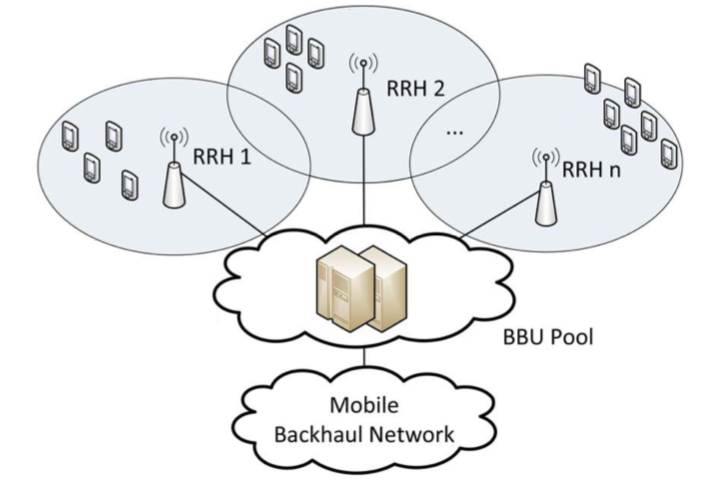
\includegraphics[width=0.6\textwidth]{images/cran}
	\caption{C-RAN}
	\label{fig:cran}
\end{figure}

\subsection{Objectives and performance indexes}
The objective of the study is to determine if and under which conditions it is better to perform packet compression or not.
For a correct evaluation of the system will be taken as reference the mean end-to-end delay of packets.

\newpage

\section{Model}
The model based to the queueing theory is shown in Figure~\ref{fig:model}.
We have $ N + 1 $ service centers, one represents the BBU with its interarrival rate $ \lambda_{bbu} $, which corresponds to the external arrival rate $ \gamma $ of the whole system, and service rate $ \mu_{bbu} $, the other N ones represent the RRHs with their $ \lambda_{rrh} $ and $ \mu_{rrh} $. Packets that leave the BBU have the same probability to reach the i-th RRH (i.e. $ \pi_{i} = \pi \text{ } \forall i $).
\begin{figure}[h]
	\centering
	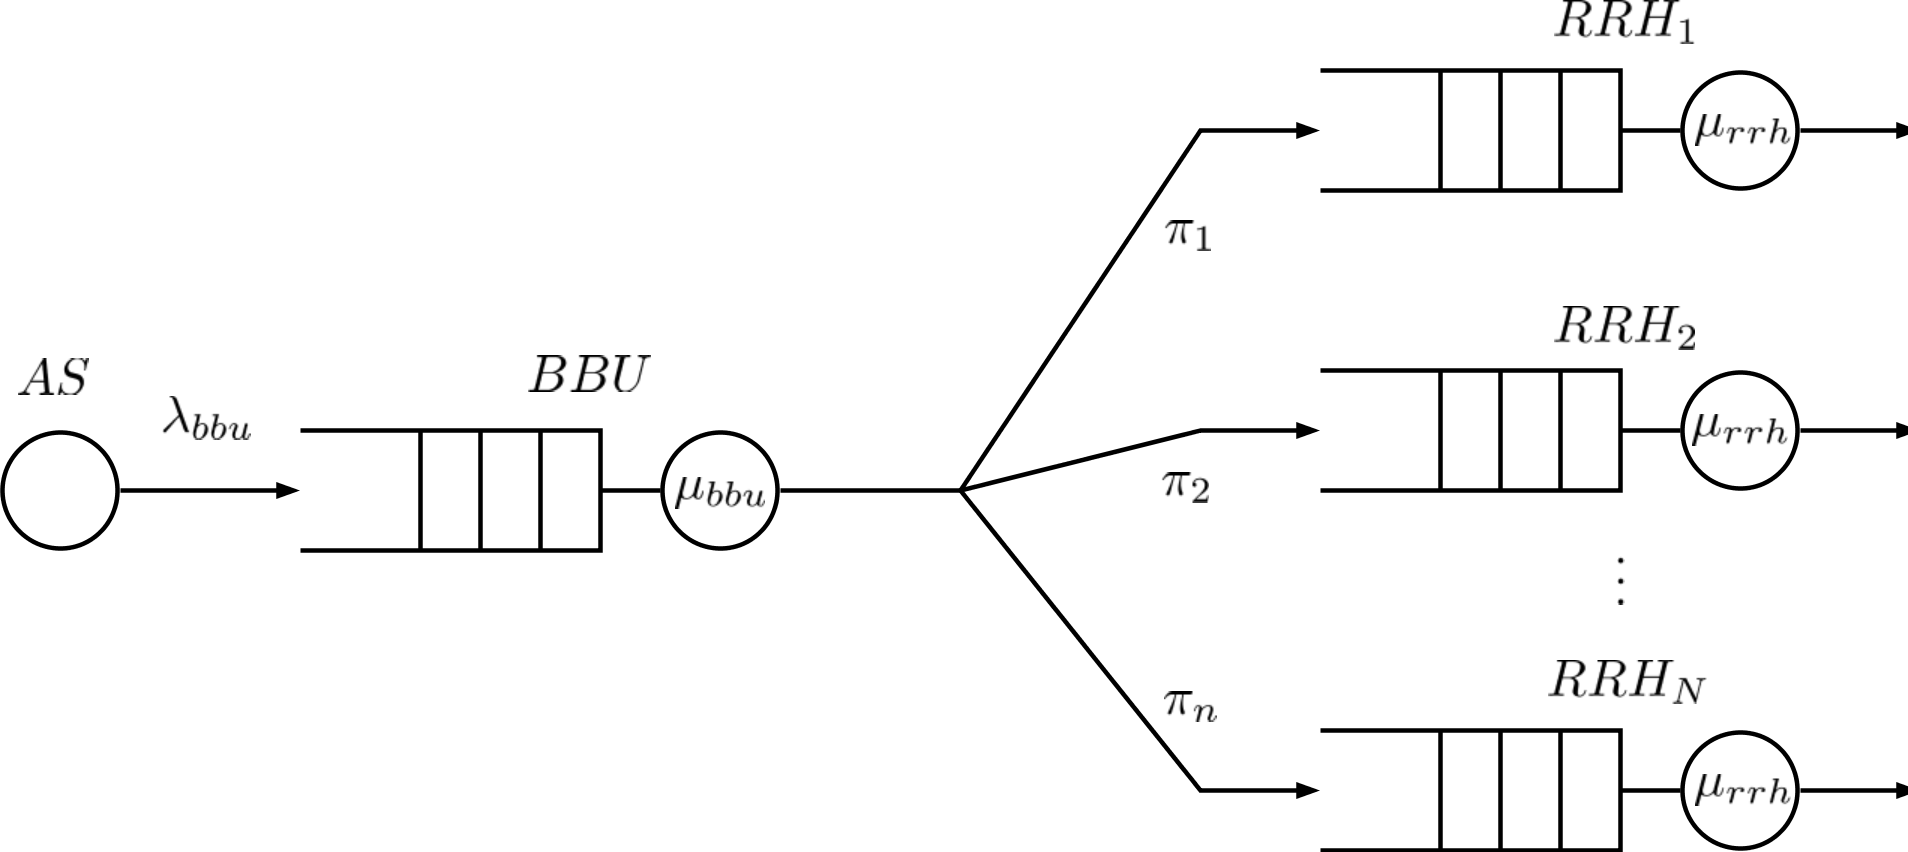
\includegraphics[width=0.6\textwidth]{images/model}
	\caption{Queueing network model}
	\label{fig:model}
\end{figure}

We make some semplifications which do not affect the final results:
\begin{itemize}
    \item time to reach the next service center is negligible;
    \item BBU switching time (time needed to change the output gate) is negligible;
    \item compression time on BBU is negligible;
    \item packets are not corrupted;
    \item no packet loss at the buffers (infinite buffers).
\end{itemize}

With these assumptions, we can compute the end-to-end delay in the following way:

% METTERE I MEAN?

$$ T_{delay} =  T_{waiting\_bbu} + T_{transmission} + T_{waiting\_rrh} + T_{decompression} $$

where 

$$ T_{transmission} = \frac{1}{\mu_{bbu}} = \frac{s}{X} $$

and

$$ T_{decompression} = \frac{1}{\mu_{rrh}} = C \cdot 50ms $$

\subsection{Validation}
The simulator has been validated through a comparison with a queueing theory model of the system.

The system has been modelled as an Open Jackson Network because all the hypotheses are verified since external arrivals are poissonian and routing probabilities are state-independent because they are uniform as specified in the requirements.

\subsubsection{Stability conditions}
In order to compute the stabilty conditions we have to distinguish between the two cases. In all equations we use the mean value of parameters and factors.

In case A we have to respect only one condition regarding the BBU. Indeed, on the RRHs we will never have queues because when the packet arrives it is immediately consumed.
Hence, the stability condition for the whole system, without compression, is the following:

$$ \lambda_{bbu} < \mu_{bbu}, \quad \lambda_{bbu} = \frac{1}{t}, \quad \mu_{bbu} = \frac{X}{s}$$

\begin{equation} \label{eq:rho-bbu}
\rho_{bbu} = \frac{\lambda_{bbu}}{\mu_{bbu}} = \frac{s}{t \cdot X} < 1
\end{equation}

Note that $s$ represents the number of bytes that the BBU has to transmit:
$$s = s_{original}\cdot(1-\frac{C}{100})$$
where $ s_{original} $ is the mean original packet size not compressed.

In case B we have also to take in account the stability condition on the RRHs because, in a system that foresees the use of some compression algorithm, the RRH service time is not null and depends on the compression percentage. In the BBU, since compression time is negligible, its stability condition does not change. 

Moreover, we have to consider the arrival rate on RRHs.
We have to guarantee that the latter is poissonian. If we consider just one RRH, the model can be seen as a tandem QN which respects Burke's theorem, since queues are infinte by our semplifications. Hence, the arrival rate at the RRH is a Poisson process with rate $ \lambda_{bbu} $ regardless of the BBU service rate, that, in our simulations, will be both exponential and lognormal. 
In a system with more than one RRH, any probabilistic splitting of a Poissonian process still originates Poissonian processes. Each RRH arrival rate will depend on the $ \lambda_{bbu} $ and on the number of remote radios as follows:

$$ \lambda_{rrh} = \lambda_{bbu} \cdot \pi = \frac{1}{t \cdot N} $$

$$ \mu_{rrh} = \frac{1}{C \cdot k}, \quad k = 50ms $$

\begin{equation} \label{eq:rho-rrh}
\rho_{rrh} = \frac{\lambda_{rrh}}{\mu_{rrh}} = \frac{C \cdot k}{t \cdot N} < 1
\end{equation}

Hence, using the result obtained in \ref{eq:rho-bbu}, the final stability condition for case B is:

$$ \begin{cases} \rho_{bbu} = \frac{s}{t \cdot X} < 1 \\ \\ \rho_{rrh} = \frac{C \cdot k}{t \cdot N} < 1 \end{cases} $$

with steady state probability, either on BBU and RRHs, equal to:

$$ p_{n} = \rho^n \cdot (1 - \rho) $$

Note that the steady state probability on each RRH and on the BBU is equal to an M/M/1.

\subsection{Statistics for validation}
In order to validate our model we have used the following perfomance indexes taken from the queueing theory:
\begin{equation}
E[N_{bbu}] = \frac{\rho_{bbu}}{1 - \rho_{bbu}} = \frac{s}{X \cdot t - s} \qquad E[R_{bbu}] = \frac{E[N_{bbu}]}{\lambda_{bbu}} =  \frac{s \cdot t}{X \cdot t - s}
\label{eq:response-time-bbu}
\end{equation}
\begin{equation}
E[N_{rrh}] = \frac{\rho_{rrh}}{1 - \rho_{rrh}} = \frac{C \cdot k}{t \cdot N - C \cdot k} \qquad E[R_{rrh}] = \frac{E[N_{rrh}]}{\lambda_{rrh}} = \frac{C \cdot k \cdot t \cdot N}{t \cdot N - C \cdot k}
\label{eq:response-time-rrh}
\end{equation}



The successful comparison between these equations and the simulator results assure us that we are working on a correct model for our system.

\section{Simulator implementation}
The simulator consists of four modules as shown in Figure~\ref{fig:simulator}:
\begin{itemize}
  \item \texttt{As}: it creates/produces a packet flow according to the interarrival time sending them to the BBU;
  \item \texttt{Bbu}: it forwards the packets received from the AS to the RRH, compressing the packet if it has to;
  \item \texttt{Rrh}: it decompresses the packet, if it was compressed, and sends it to the collector for the delay statistics;
  \item \texttt{Collector}: it handles the delay statistics.
\end{itemize}

\begin{figure}[h]
    \centering
    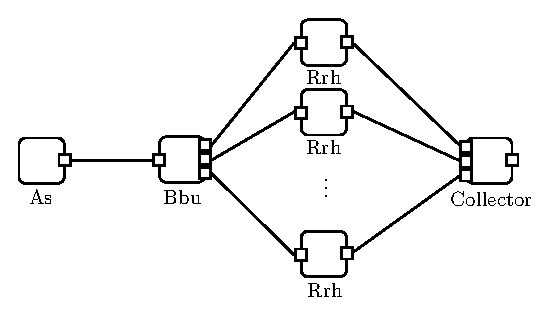
\includegraphics[width=0.6\textwidth]{images/simulator}
    \caption{Simulator architecture}
    \label{fig:simulator}
\end{figure}

\subsection{Application Server (AS)}
The As module has to perform cyclically the following operations:
\begin{itemize}
    \item[1.] it creates a new packet with the \texttt{id}, the packet size \texttt{size} taken either from an exponential distribution or a lognormal one, the destination \texttt{dest} taken from an uniform distribution, the creation time \texttt{created\_at};
    \item[2.] it sends the packet to the BBU;
    \item[3.] it waits according to the interarrival time \texttt{t} taken from an exponential distribution.
\end{itemize}

\subsection{Baseband Unit (BBU)}
When the Bbu module receives a packet from the AS it has to do the following actions:
\begin{itemize}
    \item[1.] if it is idle, it processes the packet immediately, otherwise the packet will be queued and served using a FIFO policy;
    \item[2.] it processes the packet deciding whether the packet must be compressed or not and transmitting it to the proper RRH;
    \item[3.] if there are any other packets in the queue, the first of them is pulled off from the buffer and served, otherwise it waits for the next packet.
\end{itemize}

\subsection{Remote radio (RRH)}
When one of the N RRHs receives a packet from the BBU, it acts as follows:
\begin{itemize}
    \item[1.] if it is idle, it processes the packet immediately, otherwise the packet will be queued and served using a FIFO policy;
    \item[2.] it processes the packet deciding whether the packet must be decompressed or not and transmitting it to the Collector;
    \item[3.] if there are any other packets in the queue, the first of them is pulled off from the buffer and served, otherwise it waits for the next packet.
\end{itemize}


\subsection{Collector}
The Collector module collects all the packets coming from the RRHs and deals with the end-to-end delay statistics.

\section{Verification}
The simulator has been verified in order to check for memory leaks and bugs.
For the first ones we have used Valgrind tool, whereas, for bugs, we have done some simulations with known results.

We have set proper values, for both \texttt{warmup-time} and \texttt{simulation-time-limit}, according to some simulation results.
\begin{figure}[h]
	\centering
	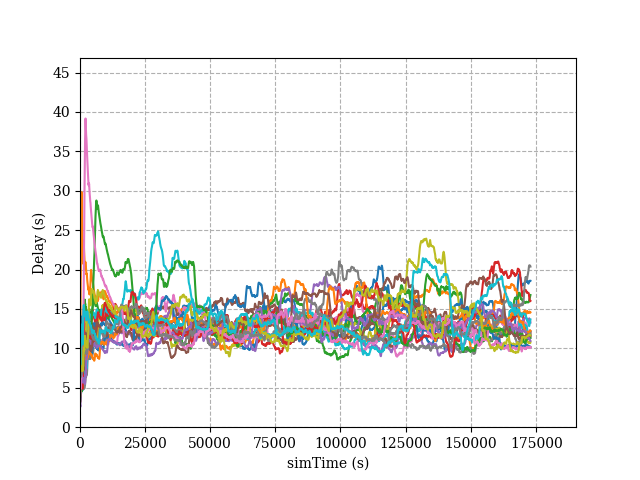
\includegraphics[width=0.6\textwidth]{images/warm-up}
	\caption{Warm-up study}
	\label{fig:warm-up-study}
\end{figure}

We have estimated the \texttt{warmup-time} applying the sliding window average (i.e. windowSize = 10000) to the end-to-end delay values obtained from 20 independent repetitions of our highest value of $ \rho_{bbu} $ (0.9). The same method will be applied to every simulation.

In Figure~\ref{fig:warm-up-study} it is shown that, in this illustrative case, a good value for \texttt{warmup-time} is around 50000 seconds, where the initial transient is over and the steady state is reached. 

The value for the \texttt{simulation-time-limit} has been chosen in order to have enough results for statistics (i.e. 2 days of simulation time).

\section{Experiments}
We will analyse separately the two cases described in Section~\ref{sec:introduction} either with exponential and lognormal distribution, the latter only for the packet size.
We will take in account scenarios with at least 2 remote radios, because a system with only one remote radio is not interesting to analyse. For each case we have done 20 different repetitions for every single scenario.
The number of repetitions are enough in order to have a level of 99\% confidence. 

\subsection{Case A - Transmission without compression}
In this case the end-to-end delay could depend on two factors:
\begin{itemize}
	\item \texttt{X}, chosen such as $ \rho_{bbu} $, computed as in \ref{eq:rho-bbu}, will assume values from 0.1 to 0.9 increased by 0.1;
	\item \texttt{N}, with prefixed values of 2, 5, 10.
\end{itemize}

\subsubsection{Exponential}
In Figure~\ref{fig:case-a-exp}, as we expected, we can see that the end-to-end delay does not depend on the number of remote radios \texttt{N} because on the RRH the service time is null, so there will be no queues and the packets will be forwarded to the cells immediately.

In fact, the three different plots (i.e. 2, 5 and 10 RRHs) overlap perfectly.
Hence, the end-to-end delay corresponds only to the BBU response time and the only factor that characterize the end-to-end delay is the BBU transmission speed \texttt{X}.


%\begin{align}
%E[R] &= E[R_{bbu}] \notag \\
%&= E[W_{bbu}] + \frac{1}{\mu_{bbu}} \notag \\
%\end{align}
\subsubsection{Lognormal}
In the lognormal scenario, the probability to have packet size values greater than the mean value is higher with respect to the exponential distribution, since the latter does not provide a variance control and the size could assume both small and large values. For this reason the end-to-end delay (shown in Figure~\ref{fig:case-a-log}) has the same trend of exponential, except for the lowest value of $ \rho $ we condired, where the delay is higher than the previous analysis.

Furthermore, we can notice that the confidence interval the lowest value of \texttt{X} (i.e. $\rho = 0.9$) is wider than the exponential one. This is due to the fact that the system is sensitive to an unlucky stream of packet whose size is greater than the mean size value.


\begin{figure}
\centering
\begin{subfigure}{.5\textwidth}
  \centering
  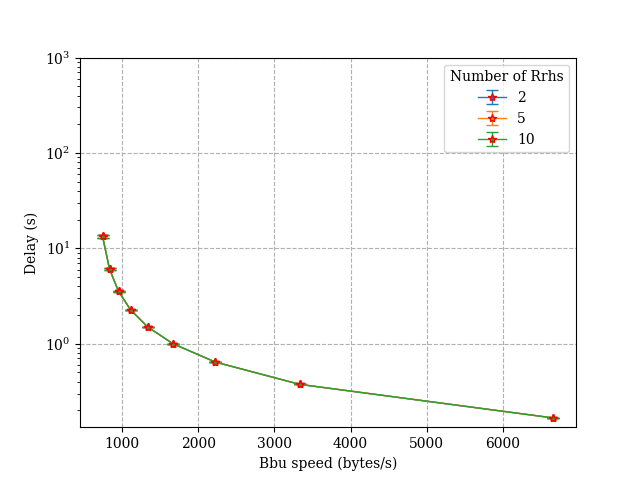
\includegraphics[width=\linewidth]{images/case-a-exp}
  \caption{Exponential distribution}
  \label{fig:case-a-exp}
\end{subfigure}%
\begin{subfigure}{.5\textwidth}
  \centering
  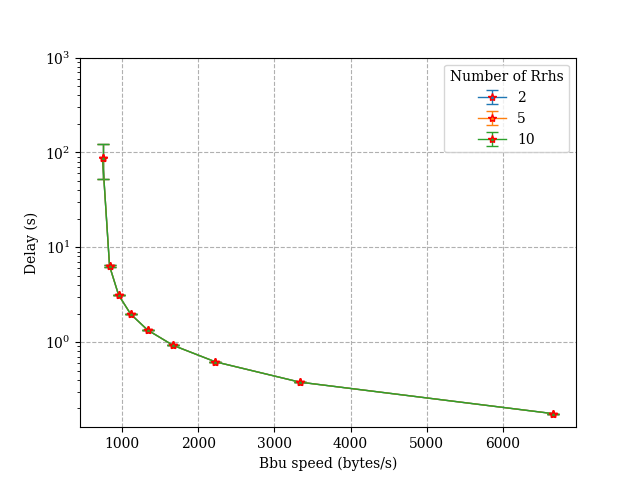
\includegraphics[width=\linewidth]{images/case-a-logn}
  \caption{Lognormal distribution}
  \label{fig:case-a-log}
\end{subfigure}
\caption{Case without compression}
\label{fig:case-a}
\end{figure}

Of course, also in this case, the only meaningful scalable factor is the BBU transmission speed.
\bigbreak

\subsection{Case B - Transmission with compression}
In addition to the factors of case A, in case B we have a further factor to take in account: the compression percentage. Hence, the set of factors becomes:

\begin{itemize}
	\item \texttt{X}, that will assume the same values of case A, but we have to consider that now $ \rho_{bbu} $ depends on the compression percentage because of the smaller number of bytes transmitted. We have chosen these values for the sake of a correct comparison between the two cases.
	\item \texttt{C}, with values ranging from 10 to 90. 
	\item \texttt{N}, with values ranging from 4 to 30. These bounds have been set in order to have $\rho_{rrh}$ values ranging from 0.1 to 0.9 for \texttt{C} equal to 90\%, maximum workload on the RRHs, considering that $\texttt{N} \propto \frac{C}{\rho_{rrh}}$.	
\end{itemize}


\subsubsection{Exponential}
By Burke's theorem consequences we can assert that the response time of the whole system can be studied splitting it into the BBU and RRH response times:

\begin{figure}[H]
  \centering
  \begin{subfigure}{.5\textwidth}
  	\centering
  	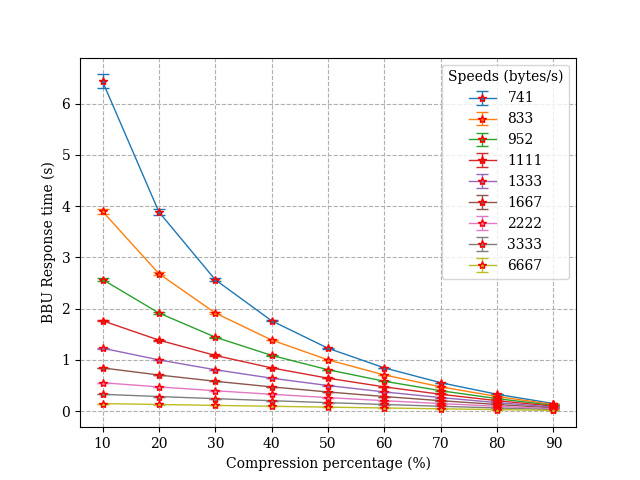
\includegraphics[width=\linewidth]{images/c-vs-response-time-bbu}
  	\caption{BBU response time in relation to \texttt{C} and \texttt{X}}
  	\label{fig:c-vs-response-time-bbu}
  \end{subfigure}%
  \begin{subfigure}{.5\textwidth}
    \centering
    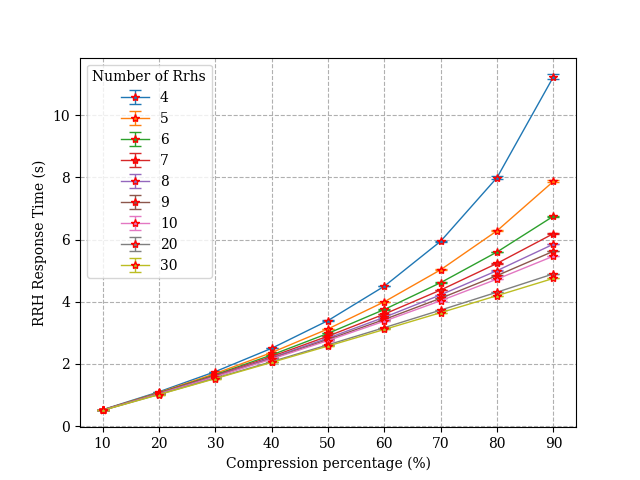
\includegraphics[width=\linewidth]{images/c-vs-response-time-rrh}
    \caption{RRH response time in relation to \texttt{C} and \texttt{N}}
    \label{fig:c-vs-response-time-rrh}
  \end{subfigure}
  \caption{Response time}
  \label{fig:response-time}
\end{figure}
\begin{equation}
E[R] = E[R]_{bbu} + E[R]_{rrh}
\end{equation} 
As we can see in \ref{eq:response-time-bbu}, the mean BBU response time does not depend on \texttt{N}, hence we can analyse its behaviour in relation to \texttt{C} and \texttt{X}.
As we expected, as \texttt{C} goes up, the BBU response time decreases because it transmits a lower number of bytes and for slower speeds the benefits obtained through compression are valuable. On the other hand when \texttt{X} is high there are almost no differences in having high or low compression percentage. %The resulting delay reduction in compressing at \texttt{X} = 6667 bytes/s is only the 2\% of the reduction at \texttt{X} = 741 bytes/s.%
From another point of view, as \texttt{C} increases, \texttt{X} becomes less and less influential to the point that, for \texttt{C} equal to 90\%, becomes completely irrelevant.
\begin{figure}[H]
	\centering
	\begin{subfigure}{.5\textwidth}
		\centering
		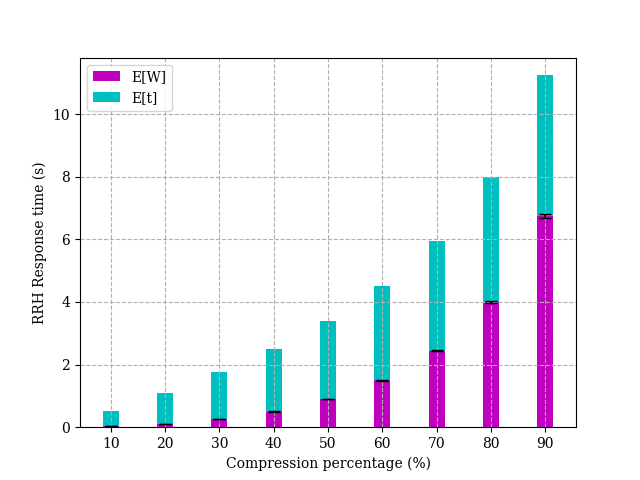
\includegraphics[width=\linewidth]{images/response-time-rrh-ratio-4}
		\caption{4 RRHs}
		\label{fig:response-time-rrh-ratio-4}
	\end{subfigure}%
	\begin{subfigure}{.5\textwidth}
		\centering
		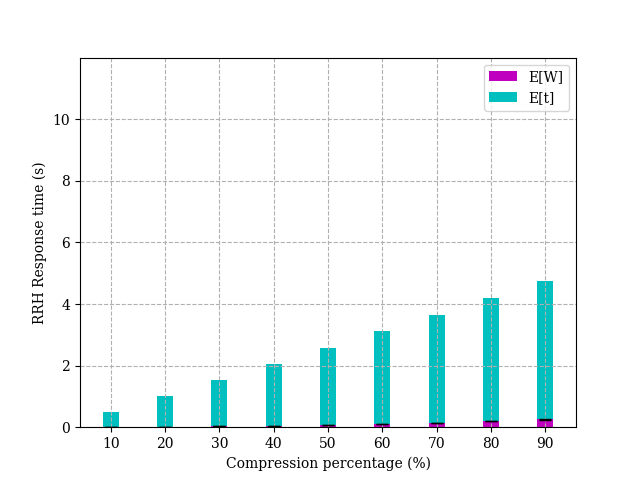
\includegraphics[width=\linewidth]{images/response-time-rrh-ratio-30}
		\caption{30 RRHs}
		\label{fig:response-time-rrh-ratio-30}
	\end{subfigure}
	\caption{}
	\label{fig:response-time-rrh-ratio}
\end{figure}
In the same way the mean RRH response time does not depend on \texttt{X}, hence we can analyse its behaviour in relation to \texttt{C} and \texttt{N}.
As \texttt{C} goes down, the RRH response time decreases because the service time is faster and the number of RRHs tends to be irrelevant. Otherwise, for high values of \texttt{C}, the longer service time needed gains more benefits from an high \texttt{N} because of the workload uniform redistribution, as shown in Figure~\ref{fig:response-time-rrh-ratio}.
The main limiting factor on the RRHs is the decompression algorithm used, which has complexity O(1) because, at the same \texttt{C}, it will always take the same time $ S $, regardless of the packet size to decompress.
\begin{figure}[H]
	\centering
	\begin{subfigure}{.5\textwidth}
		\centering
		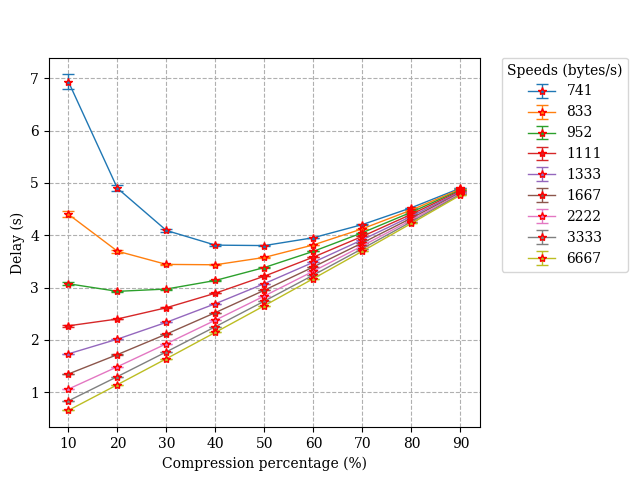
\includegraphics[width=\linewidth]{images/c-vs-delay-n-30}
		\caption{}
		\label{fig:c-vs-delay-n-30}
	\end{subfigure}%
	\begin{subfigure}{.5\textwidth}
		\centering
		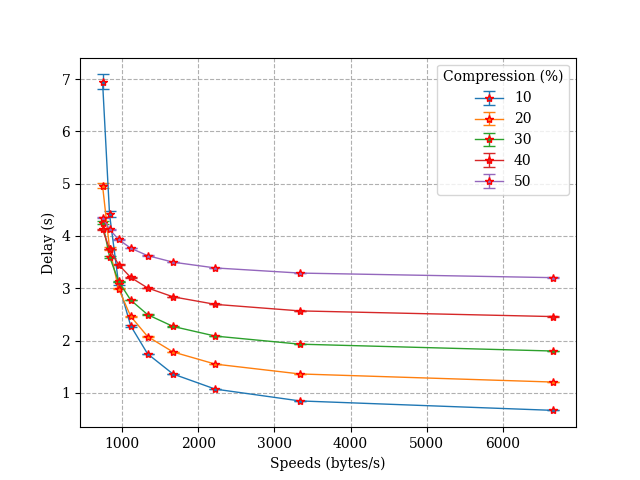
\includegraphics[width=\linewidth]{images/s-vs-delay-n-30}
		\caption{}
		\label{fig:s-vs-delay-n-30}
	\end{subfigure}
	\caption{}
	\label{fig:delay-n-30}
\end{figure}

While the BBU response time decreases as \texttt{C} increases, the RRH response time behaves in the opposite way. For this reason we can not assert a priori whether increasing or decreasing \texttt{C} brings advantages to the system, so we have to analyse when the benefits taken from the size reduction on the BBU are greater than the damages brought by RRH service time. Hence, we need a global view of the system through the end-to-end delay analysis, fixing factors at representative values.

First of all we fix \texttt{N} equal to 30 because, as we have already seen from Figure~\ref{fig:response-time-rrh-ratio-30}, the RRH waiting time is negligible for every \texttt{C} and we are in the best scenario from the RRH point of view. We do this beacuse if, in this case, we do not have any advantages on compressing, we are sure that there will neither be in worse cases, given that the response time has a monotonically increasing trend.


As we can see from Figure~\ref{fig:c-vs-delay-n-30}, for every considered speed values, we do not have any advantages in using compression over 50\%, because we have already crossed the point of maximum gain. 
% DIRE CHE ANCHE CON PIù PICCOLO N NON HA UN UNTILIZZAZIONE MAGGIORE DEL 40%
Moreover, from Figure~\ref{fig:s-vs-delay-n-30}, for speeds over about 1000 bytes/s, the end-to-end delay decreases as \texttt{C} decreases. For this reason we will analyse, in more details with a compression range from 10\% to 50\%, the remaining speeds whose behaviour is not defined yet.

\begin{figure}[H]
	\centering
	\begin{subfigure}{.5\textwidth}
		\centering
		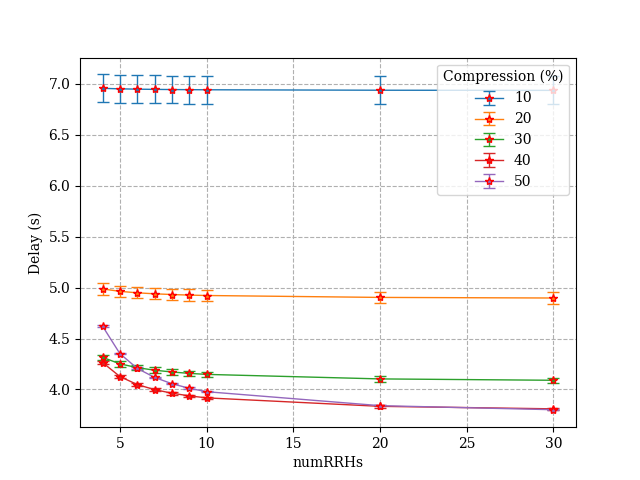
\includegraphics[width=\linewidth]{images/n-vs-delay-s-741}
		\caption{741 bytes/s}
		\label{fig:n-vs-delay-s-741}
	\end{subfigure}%
	\begin{subfigure}{.5\textwidth}
		\centering
		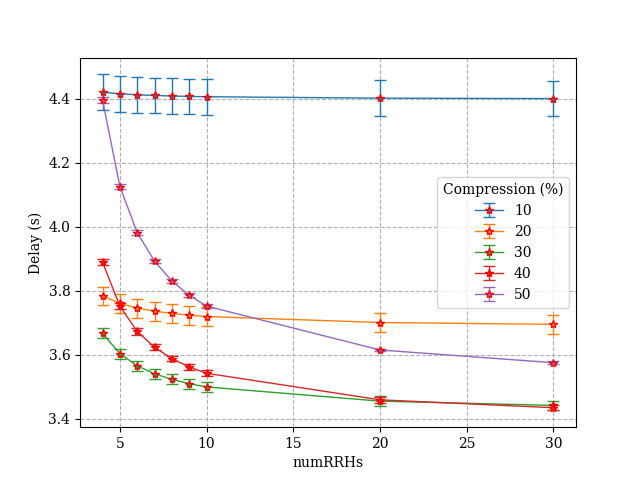
\includegraphics[width=\linewidth]{images/n-vs-delay-s-833}
		\caption{833 bytes/s}
		\label{fig:n-vs-delay-s-833}
	\end{subfigure}%
	
	\begin{subfigure}{.5\textwidth}
		\centering
		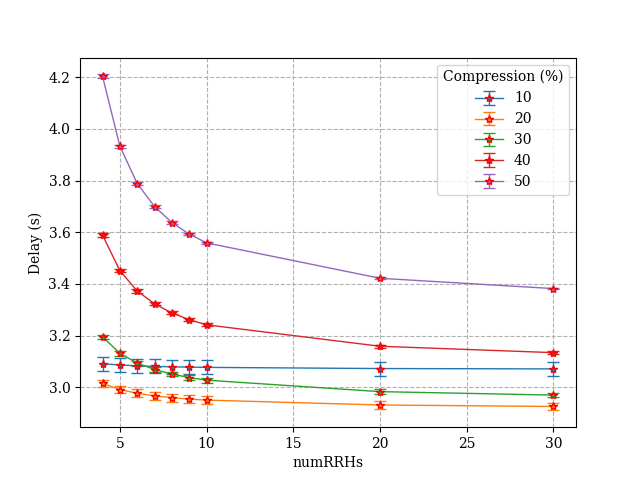
\includegraphics[width=\linewidth]{images/n-vs-delay-s-952}
		\caption{952 bytes/s}
		\label{fig:n-vs-delay-s-952}
	\end{subfigure}
	\caption{Delay in relation to \texttt{C} and \texttt{N}}
	\label{fig:n-vs-delay}
\end{figure}
These three speeds considered have the most advantages on different compression percentage. 
For the slowest speed (i.e. 741 bytes/s) the best solution is using around 40\% of compression, 30\% for the middle one, 20\% for the last one.
This trend confirm that as speed decreases, the gain on the BBU given by the best compression is higher than the leak on RRHs.
We can notice that for every speed the best compression is worth regardless the number of remote radios, ???meaning that??? the latter is the less influential factor of the system.
At the end, the main factor on which the system depends is the combination between speed and compression percentage.

\subsubsection{Lognormal}
As we have seen in case A, for $\rho \simeq 1$ (in our case \texttt{X} equal to 741bytes/s), the end-to-end delay, which is affected only by the BBU response time, assumes very high values and suffers a large variance. In case B we will not have anymore this situation due to the fact that the BBU transmits less bytes depending on \texttt{C}. Considering that $\rho_{bbu}$ is computed as in \ref{eq:rho-bbu} and \texttt{s} is reduced by \texttt{C}\%, its value (for equal \texttt{X} of case A) will be lower and the BBU will stabilize first.
\begin{figure}[h]
	\centering
	\begin{subfigure}{.5\textwidth}
		\centering
		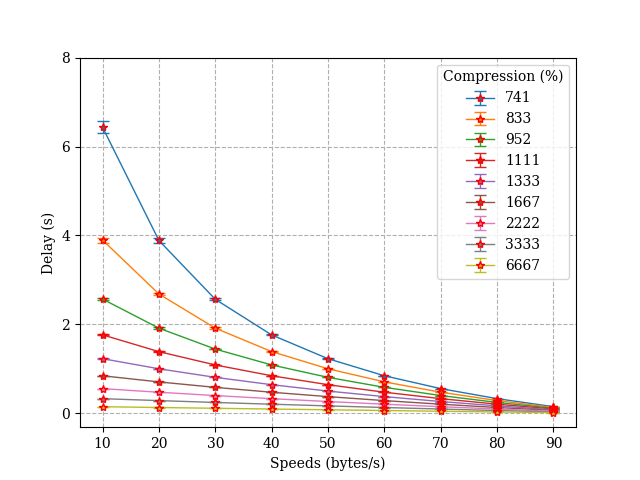
\includegraphics[width=\linewidth]{images/bbu-exp}
		\caption{Exponential}
		\label{fig:exponential-bbu-response}
	\end{subfigure}%
	\begin{subfigure}{.5\textwidth}
		\centering
		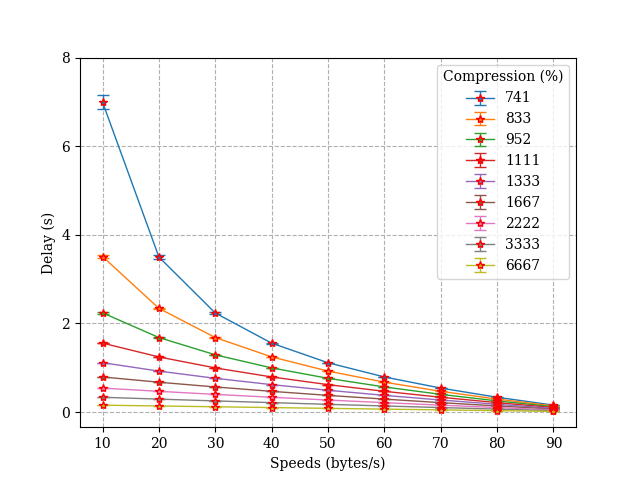
\includegraphics[width=\linewidth]{images/bbu-logn}
		\caption{Lognormal}
		\label{fig:lognormal-bbu-response}
	\end{subfigure}
	\caption{BBU response time}
	\label{fig:bbu-response}
\end{figure}
A different distribution for packet size affects only the BBU service time beacuse our system respects Burke's theorem. The RRHs will behave in the same way of the exponential distribution case. Hence, it is sufficient to study the BBU response time with packet size taken from the lognormal distribution.


When $\rho_{bbu}$ goes up the performance of the lognormal distribution is worse than the exponential one, instead for lower values of $\rho_{bbu}$ we have slightly shorter response times. Given the performance similarity of the two response times and the RRH behaviour independence from the BBU, we can assert that the insights made for the exponential case are valid for the lognormal case too.
\newpage
\subsection{Comparison}
In case B we took for granted that the system uses a packet compression algorithm, and we analysed which was the optimum compression range for a given speed. Now we take in account the possibility to compress or not. 

\begin{figure}[h]
	\centering
	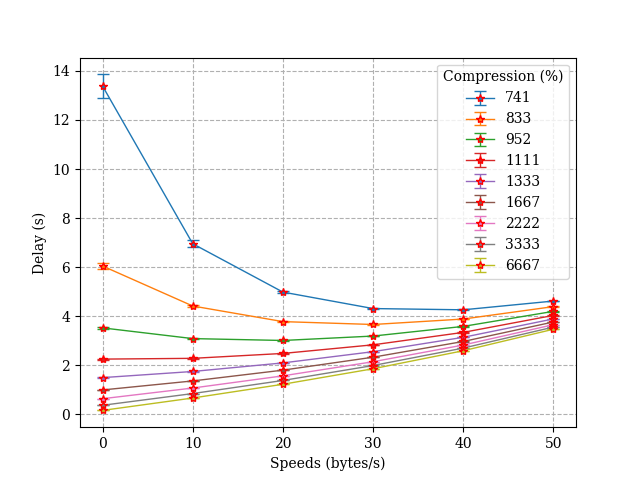
\includegraphics[width=0.5\textwidth]{images/c-vs-delay-n-4}
	\caption{Delay in relation to \texttt{C} and \texttt{X}, \texttt{N} = 4} 
	\label{fig:c-vs-delay-n-4}
\end{figure}

First, we show the worst case analysis from the RRH point of view because if it is convenient to compress at the worst case, it will be also for the better cases. 

\begin{figure}[H]
	\centering
	\begin{subfigure}{.45\textwidth}
		\centering
		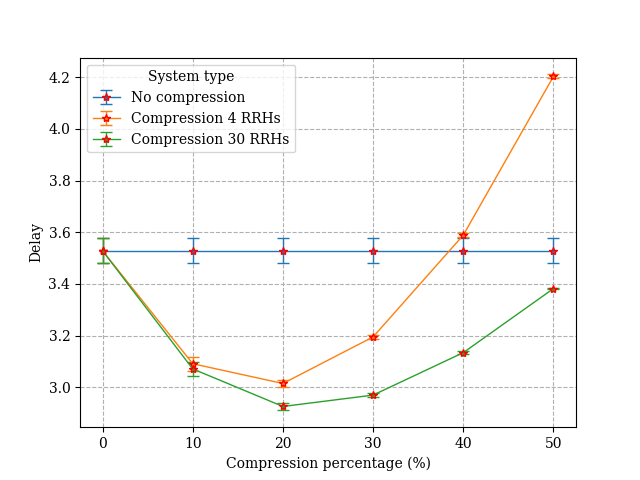
\includegraphics[width=\linewidth]{images/comp-s-952}
		\caption{952 bytes/s}
		\label{fig:comp-s-952}
	\end{subfigure}%
	\begin{subfigure}{.45\textwidth}
		\centering
		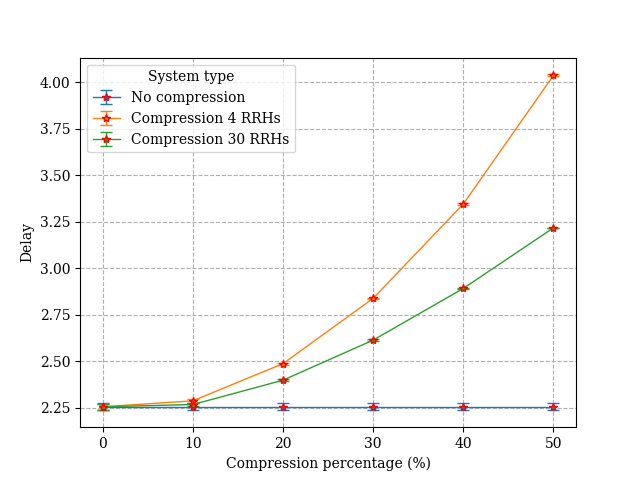
\includegraphics[width=\linewidth]{images/comp-s-1111}
		\caption{1111 bytes/s}
		\label{fig:comp-s-1111}
	\end{subfigure}
	\begin{subfigure}{.45\textwidth}
		\centering
		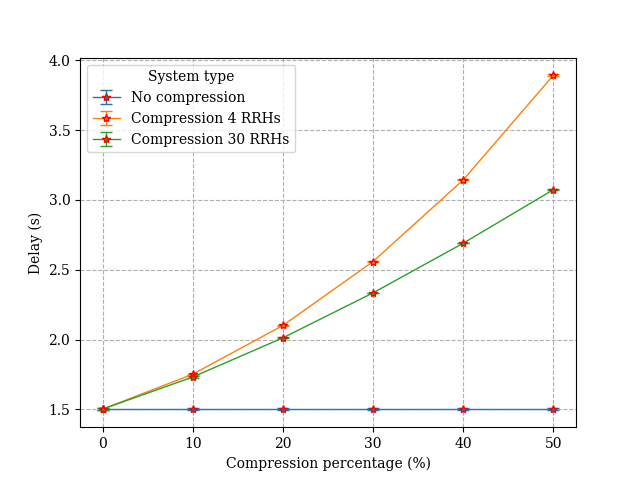
\includegraphics[width=\linewidth]{images/comp-s-1333}
		\caption{1333 bytes/s}
		\label{fig:comp-s-1333}
	\end{subfigure}
	\caption{Delay in relation to \texttt{C} and \texttt{N} = \{4, 30\}}
	\label{fig:compress-s}
\end{figure}

We took 4 RRHs as our worst case because, as we have seen in Figure~\ref{fig:c-vs-response-time-rrh}, in case of compression with 4 RRHs we have higher delays.

For the three slowest BBU speeds exists at least one \texttt{C} value that grants benefits. About \texttt{X} = 1111 bytes/s the behaviour is unclear and for this reason we analyse it in more details, paired with adjacent speeds for the sake of a correct interval comparison.


We can say that:
\begin{itemize}
	\item For \texttt{X} = 952 bytes/s we can always find a non-null \texttt{C} value which gives a shorter delay in comparison to the one obtained with no compression.
	\item For \texttt{X} = 1111 bytes/s we can not state with a 99\% confidence level whether is better to do compression or not.
	\item For \texttt{X} = 1333 bytes/s it is clear that we will never have advantages in using this compression algorithm. Since as \texttt{X} goes up the benefits of compression are less relevant, we can extend this insight to higher BBU speeds. 
\end{itemize}
Hence, for the considered speed values, we can assert that it is not advantageous to choose this compression algorithm if the system setup foresees a BBU transmission speed above or equal to 1333 bytes/s, independently from the number of RRHs.
\section{Conclusions}
This project analysed a CRAN system which can adopt a compression/decompression algorithm whose compression time is null and decompression time depends on the percentage adopted.\\
Thus we studied the trend of the mean end-to-end delay in relation to \texttt{C}: 
\begin{itemize}
	\item For lower values of \texttt{C} it is more convenient increasing \texttt{X} instead of \texttt{N}. Indeed, for $\texttt{C} = 0 $ the number of remote radios is irrelevant.
	\item For high values of \texttt{C} it is more convenient increasing \texttt{N} instead of \texttt{X}. This is true for \texttt{N} up to 30, after that increasing the number of remote radios brings meaningless improvements.
\end{itemize}
For the range of analysed values, the benefits brought by compression can be appreciated only at lower BBU transmission speeds where the time gained by size reduction is greater than the time spent on the RRH because of decompression. Increasing the number of RRH, thus decreasing the workload on them, the value of \texttt{C}, that gives the shortest end-to-end delay, increases.



\end{document}